\documentclass[11pt]{article} 

\usepackage{deauthor,times,graphicx}
%\usepackage{url}
\usepackage{hyperref}



\begin{document}

Machine learning is rapidly maturing into an engineering discipline at the center of a growing range of applications.
This widespread adoption of machine learning techniques presents new challenges around the management of the data, code, models, and their relationship throughout the machine learning life-cycle.
In this special issue, 
% of the Data Engineering Bulletin 
we have solicited work from both academic and industrial leaders 
% in the data engineering community that 
who are exploring how data engineering techniques can be used to address the challenges of the machine learning life-cycle.



\iffalse
\begin{figure}[h]
\centering
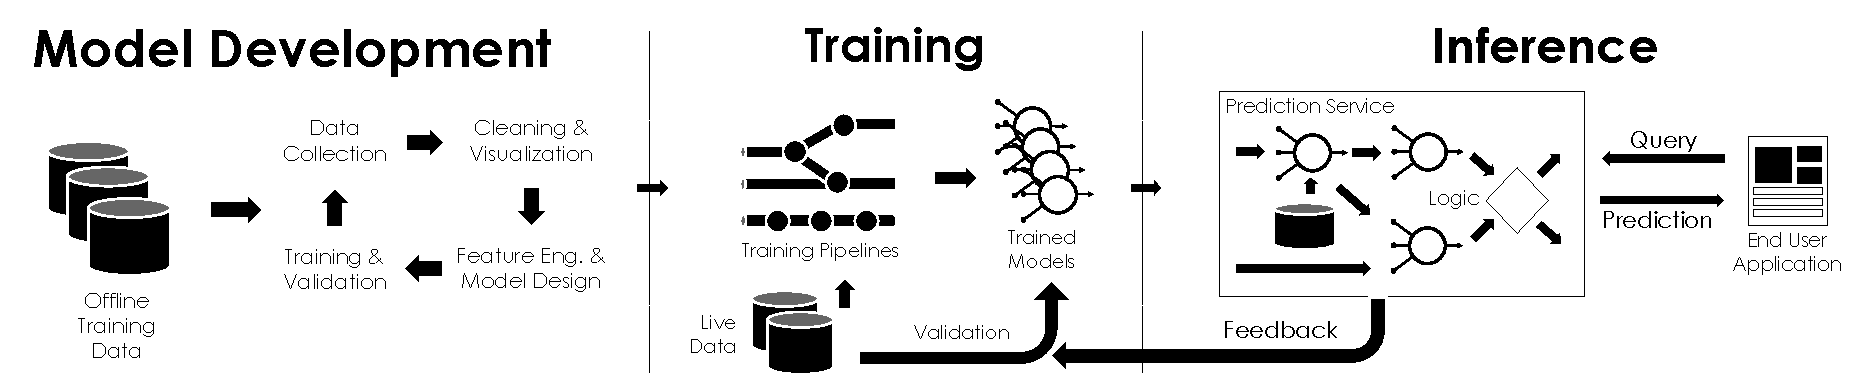
\includegraphics[width=\textwidth]{letters/pipeline.pdf}
\caption{\small \textbf{Machine Learning Life-cycle.} A simplified depiction of the key stages of a machine learning application.}
\label{fig:mllc}
\end{figure}
\fi


The machine learning life-cycle (Fig.~\ref{fig:mllc}) spans not only the model development but also production training and inference.
Each stage demands different skills (e.g., neural network design, data management, and cluster management) and imposes different requirements on the underlying systems.
Yet there is an overwhelming need for unifying design principles and technologies to address pervasive problems including feature management, data provenance, pipeline reproducibility, low-latency serving, and prediction monitoring just to name a few.


There has been a flurry of recent progress in systems to aid in managing the machine learning life-cycle.  
Large industrial projects like 
FB Learner Flow 
% \href{https://code.fb.com/core-data/introducing-fblearner-flow-facebook-s-ai-backbone/}{FB Learner Flow}
from Facebook, 
Michelangelo 
% \href{https://eng.uber.com/michelangelo/}{Michelangelo} 
from Uber, and 
TFX 
% \href{https://www.tensorflow.org/tfx/}{TFX} 
from Google have received considerable recent attention.  
In this issue, we have solicited papers from several recent industrial and academic projects that have received slightly less attention.


The first paper provides an overview of several real-world use cases and then outlines the key conceptual, data management, and engineering challenges faced in production machine learning systems.
% Rather than advocating a single system, this work describes some design principles that can inform potential solutions.
The second and third papers explores the challenges of model management and provenance across the machine learning life-cycle.
They motivate the need for systems to track models and their meta-data to improve reproducibility, collaboration, and governance. 
% expands upon the machine learning life-cycle 
% to include: data preparation, feature engineering, model training, deployment, and maintenance
% and explores the challenges of model 
The second paper introduces, ModelDB, an open-source system for model management and describe some of the functionality and design decisions. 
The third paper describes a related system, ProvDB, that uses a graph data model to capture and query fine-grained versioned lineage of data, scripts, and artifacts throughout the data analysis process.
The fourth paper describes, MLFlow, a new open-source system to address the challenges of experimentation, reproducibility, and deployment. 
This work leverages containerization to capture the model development environment and a simple tracking API to enable experiment tracking.
% The extensible model containerization enables model developers to more easily collaborate around modeling environments and then deploy model containers.
The fifth paper focuses on inference and explores the challenges and opportunities of serving white-box prediction pipelines.  
Finally, we solicited a summary of the recent Common Modeling Infrastructure (CMI) workshop at KDD 2018, which provides a summary of the keynotes and contributed talks.

The work covered here is only a small sample of the emerging space of machine learning life-cycle management systems. 
We anticipate that this will be a growing area of interest for the data engineering community.


% In contrast to the containerization of pipelines in MLFlow, the Microsoft team leverage knowledge about the internal of the prediction pipeline to more efficient serve predictions. 



\end{document}


